\chapter{Analisi}

\section{Descrizione e requisiti}
Il software mira alla costruzione di una versione virtuale del famoso gioco da tavolo \href{https://it.wikipedia.org/wiki/Monopoly}{Monopoly}. 
Quest’ultimo è un gioco di società nel quale più giocatori a turno lanciano i dadi e muovono le proprie pedine su un tabellone 
composto da caselle di cui la maggior parte sono proprietà, ovvero dei terreni acquistabili dai giocatori.
Lo scopo del gioco è di creare un monopolio aumentando i beni o il denaro posseduto. 
Per fare ciò durante la partita i giocatori possono acquistare le proprietà sulle quali capita la propria pedina pagando una somma alla banca, 
una volta acquistate il giocatore può anche decidere se eventualmente migliorarle.
Se la pedina di un giocatore finisce su una proprietà in possesso di un suo avversario allora sarà costretto
a pagargli una somma di denaro per poter transitare su un terreno non suo, in questo caso si dice che il giocatore
paga l'affitto per la proprietà.\newline
Sul tabellone saranno presenti anche delle caselle speciali: le più importanti sono il parcheggio e la prigione che
impediscono al giocatore di muoversi per un determinato numero di turni e le caselle imprevisti e probabilità che 
richiedono al giocatore di pescare una carta dal mazzo degli imprevisti e delle probabilità e seguire le 
istruzioni scritte sulla carta.\newline
L’obiettivo è mandare gli altri giocatori in bancarotta, e dunque condurli alla sconfitta, cercando di fargli spendere
più denaro possibile. Le pedine dei giocatori sconfitti vengono rimosse dal tabellone e i loro 
beni revocati, si vince rimanendo l'ultimo giocatore sul tabellone.\newline
Il software permetterà di creare e giocare un partita con un determinato numero di giocatori dallo 
stesso terminale.


\subsection{Requisiti funzionali}
\begin{itemize}
    \item Il gioco potrà essere giocato su uno stesso dispositivo da un minimo di 2 giocatori ed un massimo di 6. L'utente
    potrà impostare altre opzioni di configurazione relative al gioco prima di avviare la partita come il nome dei giocatori e 
    la modalità di gioco.
	\item Il giocatore, durante il proprio turno, potrà tirare i dadi per far muovere la propria pedina sul tabellone di un numero di 
    caselle corrispondente alla somma dei dadi lanciati.
	\item Il giocatore, dopo aver tirato i dadi, avrà la possibilità di acquistare la proprietà sulla quale 
    è capitata la sua pedina, se questa proprietà non appartiene a nessuno. 
    Se la proprietà è già posseduta da qualcun altro il giocatore che vi capita sopra dovrà pagare l’affitto al proprietario 
    per poter continuare a giocare.
    \item Se il giocatore finisce sopra la casella speciale parcheggio la sua pedina
    dovrà rimanere ferma per un turno.
    \item Se il giocatore viene messo in prigione, perchè è capitato sulla casella \say{Vai in prigione},
    dovrà rimanere fermo sulla casella \say{Prigione} per 3 turni. Ogni turno gli verrà concessa la possibilità di liberarsi lanciando i dadi
    e provando a fare un doppio come risultato.
    \item Se il giocatore finisce sopra una casella imprevisti o probabilità allora verrà pescata una carta effetto
    o dal mazzo imprevisti o dal mazzo probabilità. La carta appunto descrive un effetto che va ad agire e modificare gli
    elementi del gioco (tabellone, pedine, proprietà, denaro posseduto\dots). L'effetto eseguito è specifico della carta,
    al giocatore verrà mostrata una descrizione testuale dell'effetto e poi il sistema ne farà partire l'esecuzione.
    \item La pedina del giocatore potrà finire su altre caselle speciali con un effetto specifico che si attiverà o al 
    passaggio (casella Start) o se ci finisce esattamente sopra (casella tasse e altre)
    \item Nel corso della partita un giocatore, quando capita sulle sue proprietà, le potrà migliorare spendendo
    del denaro per posizionare delle case che elevano il costo dell’affitto o un albergo, che è come una casa 
    ma ha un costo di affitto e di acquisto maggiore.
    \item Durante il proprio turno, se lo desidera, il giocatore potrà vendere alla banca 
    proprietà ed eventuali case precedentemente costruite per riguardagnare denaro qualora fosse a rischio
    bancarotta.
\end{itemize}


\subsection{Requisiti non funzionali}
\begin{itemize}
    \item 
    Monopoly dovrà permettere agli utenti di aggiungere e 
    modificare gli effetti speciali delle carte imprevisti e probabilità
    con facilità e senza toccare il codice, bensì dandogli la possibilità di
    modificare il file di configurazione.
    \item Monopoly potrà essere giocato attraverso un'interfaccia grafica
    che dovrà essere in grado di adattarsi alle dimensioni di vari schermi.
    \item 
    Monopoly dovrà permettere agli utenti di alterare in facilità la 
    configurazione del gioco (parametri aggiuntivi di 
    configurazione della partita, struttura del tabellone e caselle che lo compongono).
    \item l'applicazione sarà in grado di girare sui principali SO desktop
\end{itemize}

\section{Modello del dominio}
Nella versione da tavolo del gioco, ai giocatori viene periodicamente concesso il proprio turno d'azione 
sulla base di una rotazione ciclica ed è durante il proprio turno che gli viene concesso di \say{giocare} e dunque
controllare i propri beni e la propria pedina.
I giocatori si coordinano tra di loro
per gestire la rotazione dei turni e arbitrare la partita verificando che ognuno rispetti le 
regole principali del gioco (controllare se un compagno ha perso, verificare che un giocatore possa terminare il suo turno, controllare casistiche particolari
in cui il giocatore deve saltare dei turni o non può muovere la propria pedina perchè magari è sulla casella prigione
o parcheggio e mantenere il conteggio dei turni da trascorrere su queste caselle\dots).\newline
Per modellare questo aspetto è stata inserita un'entità esterna che chiameremo arbitro \texttt{referee} a cui sono delegate
tutte le operazioni di coordinazione del gioco e dei suoi partecipanti. 
Queste operazioni sono:
\begin{itemize}
    \item
    Coordinare i turni dei giocatori concedendo la possibilità di giocare, 
    il giocatore potrà terminare il proprio turno solo una volta che tutte le azioni obbligatorie sono state eseguite 
    (ad esempio pagare un affitto o tirare i dadi).
    \item 
    Decretare se un giocatore è eliminato oppure no sulla base della sua situazione finanziaria,
    se il saldo del portafoglio del giocatore è in negativo perde la partita e tutti i suoi contratti di proprietà
    ritornano alla banca, disponibili per l’acquisto. 
    \item
    Decretare se il gioco è finito.
    \item Tenere il conto dei turni che un giocatore deve trascorrere bloccato nel parcheggio o nella prigione e valutare se 
    eventualmente il giocatore potrebbe liberarsi prima
\end{itemize}
Come è stato detto, a ogni giocatore \texttt{Player} viene concesso periodicamente dall'arbitro il proprio turno d’azione.
Durante il suo turno il giocatore muove sul tabellone \texttt{Board} la propria pedina \texttt{Pawn} tirando dei dadi \texttt{Dices}.
Il tabellone è composto da una serie di caselle  \texttt{Tile} disposte su un percorso chiuso. Il giocatore muove la propria pedina spostandola di 
un numero di caselle corrispondenti al tiro del dado, atterrando così su una nuova casella. 
Questa casella può essere una proprietà \texttt{Property} oppure una casella speciale \texttt{Special}, 
e sulla base di ciò cambia radicalmente l’interazione con l’utente.\newline
Le proprietà sono caselle alle quali è associato un contratto di proprietà \texttt{Title deed}. 
Quando un giocatore capita su una casella di tipo proprietà non ancora in possesso di nessun altro, può richiedere alla banca \texttt{Bank} di acquistare
il contratto associato alla suddetta proprietà.
Dopo aver pagato una somma alla banca il contratto viene consegnato al giocatore che da quel momento in poi possiederà la proprietà.
Il contratto di proprietà è un documento che descrive tutte le informazioni monetarie della proprietà.
La banca possiede tutti i contratti non acquistati.\newline
Se la proprietà su cui è capitato il giocatore era già stata comprata in precedenza da un altro allora si 
deve pagare l'affitto al proprietario. I giocatori consultano il contratto di proprietà e concordano il prezzo dell'affitto.
Il giocatore di passaggio procede poi a pagare il giocatore proprietario.\newline
Se in un turno successivo all'acquisto il giocatore capita novamente su una casella di sua proprietà può decidere se migliorarla aggiungendo case 
o alberghi acquistandoli dalla banca.
Infine ogni giocatore può rivendere alla banca un contratto e ricevere del denaro in cambio.
Ogni giocatore ha associato un conto bancario  \texttt{BankAccount} contente del denaro. Attraverso il suo conto
il giocatore compie tutte le operazioni di compravendita che comportano un addebito o prelievo di denaro (comprare/vendere contratti, pagare affitti\dots)\newline
Se il giocatore invece capita su una casella speciale si attiverà un effetto caratteristico della casella \texttt{Effect}
che avrà ripercussioni sul gioco 
(guadagno/perdita denaro, saltare un determinato numero di turni\dots). 
In particolare se si capita su una casella Imprevisti o Probabilità \texttt{Unexpected Probability} l'effetto non 
è specifico della casella stessa, ma viene letto da un mazzo di carte effetto \texttt{Deck}. 
Il giocatore pesca una carta \texttt{Card} dal mazzo, legge l'effetto e lo attiva.\smallskip\newline
Parte della difficoltà consisterà nel riadattare un dominio che non nasce intrinsecamente per un progetto software.
Monopoly infatti è un gioco da tavolo e questo si riflette in molte interazioni e funzionalità, che non sono pensate 
nell'ottica di un'architettura software (un esempio è quello dato all'inizio della sezione sulla coordinazione fra i giocatori e 
l'entità arbitro). Molte azioni nel gioco spesso comportano la comunicazione di più entità (migliorare una
proprietà ha come conseguenza un cambiamento sulla casella ma per attuarlo il giocatore deve pagare la banca facendo riferimento
al contratto di proprietà, un giocatore può passare il turno solo se ha fatto determinate azioni che dipendono non solo dalla casella in cui
si trova ma anche da chi la possiede\dots). 
Sarà quindi difficile progettare un'architettura software che permetta di rappresentare il dominio del gioco
in maniera efficace e riadattabile. 


\begin{figure}[H]
    \centering
    \makebox[1.0\textwidth]{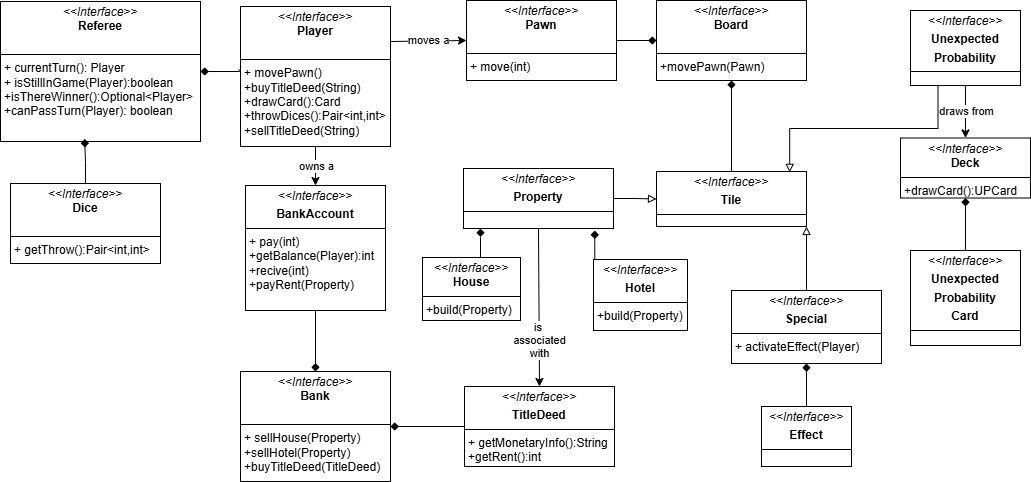
\includegraphics[width=1.3\textwidth]{img/entity_diagram.png}}	
    \caption{Schema UML dell'analisi del problema, con rappresentazione delle entità principali ed i rapporti fra loro}
	\label{img:entity_diagram}
\end{figure}
